\documentclass{article}
\usepackage[T1]{fontenc}
\usepackage{lmodern}
\usepackage{graphicx}
\usepackage{amsmath,amssymb}
\usepackage[a4paper,margin=2cm]{geometry}
\usepackage[absolute,overlay]{textpos}
\setlength{\TPHorizModule}{1mm}
\setlength{\TPVertModule}{1mm}
\usepackage[indonesian]{babel}
\usepackage{hyperref}
\setlength{\emergencystretch}{2em}
% unit: Halaman 77

\begin{document}

% === Halaman 77 (llm) ===

Bigram IH diganti menjadi MB

\vspace{10mm}

Sumber gambar: Wikipedia

% deskripsi: Ilustrasi penggantian bigram IH menjadi MB pada tabel Playfair, menunjukkan pergerakan huruf I ke M dan H ke B menggunakan tanda panah.
% bbox normalisasi: [0.2920, 0.3200, 0.6480, 0.5620]
\begin{textblock*}{74.76mm}(61.32mm,95.04mm)
\noindent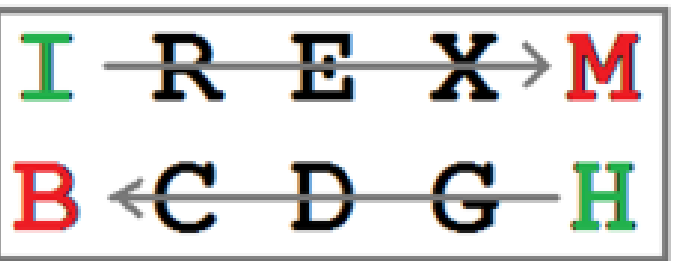
\includegraphics[width=74.76mm,height=71.87mm]{../../images/llm/page_077_img_01.png}%
\end{textblock*}

\end{document}
